\subsection{Efficient Flight Planning}

Efficient flight planning is a cornerstone of modern \gls{ATM}, particularly as global air traffic continues to grow and demands on limited airspace intensify.
Civil aviation flight plans are developed under \glspl{IFR} and must consider capacity constraints, aircraft performance limitations, and airline preferences.
However, even though flight plans are typically filed about an hour before departure, they are often not executed as planned due to factors such as adverse weather, ground congestion, and delayed arrivals  \cite{Rosenow_2021}.
These disruptions reduce airport efficiency and propagate delays throughout the air traffic network, a phenomenon often referred to as the ripple effect \cite{Ye_2024}.

Traditional \gls{ATM} research has largely focused on tactical-level solutions such as flow management, but there is growing recognition that strategic-level flight planning alsoplays a crucial role.
The works of Rosenow et al. \cite{Rosenow_2021} and Ye et al. \cite{Ye_2024} offer promising approaches to solving strategic flight planning challenges using optimisation and \gls{AI}.

Rosenow et al. \cite{Rosenow_2021} identify that conventional flight planning still heavily relies on manual processes and heuristic methods that do not fully account for the dynamic and multi-objective nature of the airspace environment.
As a result, suboptimal routes are often chosen, leading to excessive fuel consumption, extended flight times, and increased emissions.
To address this, the authors propose a multi-objective optimisation model that balances multiple goals while maintaining logical route structures and time constraints.
These goals include minimising fuel use, reducing delays, and maximising airspace utilisation.
The results demonstrate significant potential for \gls{AI}-driven models to improve operational efficiency and environmental sustainability.

Similarly, Ye et al. \cite{Ye_2024} propose a strategic flight planning framework tailored to high-demand, weather-sensitive regions in China.
Their model optimises flight scheduling with two objectives: (1) minimising total departure and arrival time offsets (\gls{FMS}), and (2) reducing strategic operational costs, including ground and airborne components (\gls{FMC}).
Using real-world data from rainy and foggy seasons at \gls{CTU}, \gls{TCZ}, and \gls{LUM}, the model showed that rerouting flights to less congested airports like \gls{LUM} during capacity constraints at \gls{TCZ} is both feasible and cost-effective.
This effectively reduces the decision-making burden on \glspl{ATCO}.

While these models highlight the effectiveness of optimisation in strategic planning, their real-world deployment faces challenges.
Current models are often constrained by limited datasets and simplifications that fail to capture the full complexity of live airspace operations.
As \gls{UAS} and \gls{UAM} begin to integrate into civilian airspace, such as those using vertiports (e.g., Munich International Airport, Figure \ref{vertiport}), the need for more robust, adaptive, and \gls{AI}-powered optimisation frameworks becomes critical.
Future systems must be capable of dynamically coordinating mixed traffic environments with both manned and unmanned aircraft, all while managing growing complexity and operational uncertainty.






% Planning flights for civil air traffic follows instrument flight rules and the development of flight plan has to comply with capacity constraints, flight performance limitations, and airline intensions. 
% Despite the flight plan is made an hour before departure, often flights are not flown as planned \cite{Rosenow_2021}. 
% This could be attribted to bad weather, congestion on airport ground, and delayed arrival of flights; all which combined further reduce the airport effiency and causes the ripple effects of delayed flights \cite{Ye_2024}. 
% Previous studies have predominantly approached \gls{ATM} from the perspective of flow management, addressing issues on a tactical level. 
% However, the balance between traffic demand and capacity has not been adequately address from the stretegic level of flight planning \cite{Ye_2024}. 
% In the following two papers we discuss here, it is about solving the optimisation problem to optimise flight route based on demand through the use of linear programming method.


% In the paper written by Rosenow et al \cite{Rosenow_2021}, it has identified that traditional flight planning approaches often rely on manual processes and heuristics
% This may not fully capture the dynamic nature of the aviation environment or consider multiple objectives simultaneously. 
% This may result flight routes to be suboptimal, leading to increased fuel consumption, longer flight times, and unnecessary emissions.
% The goal is to created a model through multi-objective optimisation approaches, to obtain optimised routing decisions, that is able to minimise fuel consumption, reduce flight time and enhance overall operational efficiency.
% The model is able to produce the optimised routing decision, and showcased the potential benefits of the new generation of air routing, including minimized fuel consumption, reduced flight time, efficient airspace capacity utilization, adherence to time windows, and logical route connectivity.


% In the paper written by Ye et al \cite{Ye_2024}, a strategic flight planning model was proposed to match the flight demand while effectively utilising existing airport resources.
% The model has two different objective functions: \gls{FMS} and \gls{FMC}, and its goals are described as follow:
% \begin{itemize}
%     \item \Gls{FMS}: to minimise the total offset of departure and arrival times for all flight, while fulfilling the requirements of the flight scheduling arrangement.
%     \item \Gls{FMC}: to reduce the strategic operating costs of flights, including ground and air operations. 
% \end{itemize}
% The model is based on flight data from \gls{CTU} to \gls{TCZ} and \gls{LUM}, both in the Yunnan province in China, during the period of rainy and foggy season from June to September.
% The destination airports have a capacity of 9 and 16 hourly capacity of planes.
% This study is able to confirm the feasibility of adjusting flight schedules of a original flight from \gls{CTU} to \gls{TCZ} to a redirected flight to \gls{LUM} (to cope with the limited airport capacity in \gls{TCZ} in case of bad weather), with small number of flights requiring replacements and at similar operating cost level.
% This shows that the model is able to make decision on behalf of \glspl{ATCO}, reducing the workload of \gls{ATCO}. 

% Despite proving that the optimisation model work successful, they are often limited by their data and constraints, as they do not fully represent all possible variables in the real world. 
% On top of that, vertiports are begining to be built in airports (example:  Munich International Airport in Figure \ref{vertiport}) and the integration of \gls{UAM} into our already congested airspace begin. 
% There will be hence a need to develop a optimision model to represent this new world. 


\begin{figure}[!ht]
    \centering
    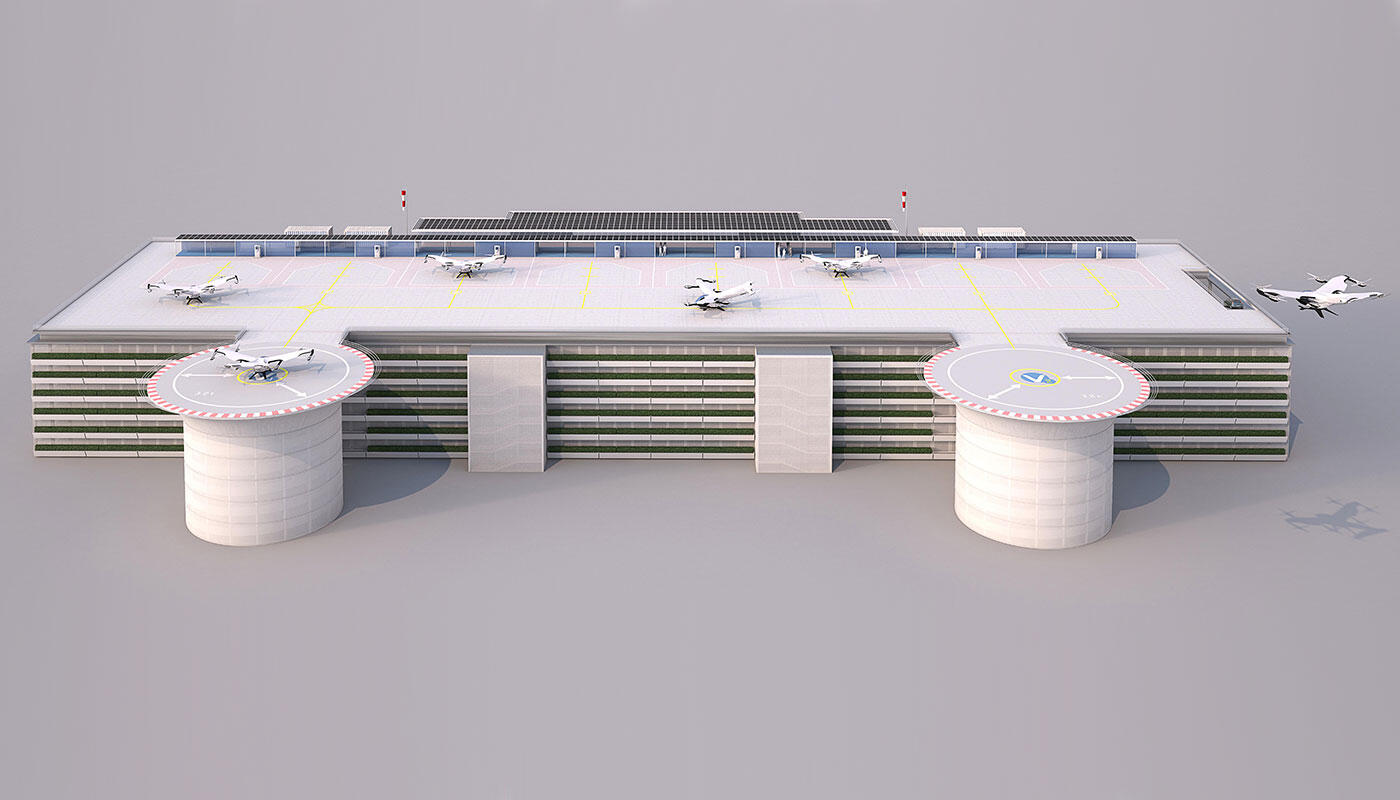
\includegraphics[width=.6\textwidth]{img/vertiport.jpeg}
    \caption{Development of vertiport on a parking garage at Munich International Airport \cite{amd_vertiport}.}
    \label{vertiport}
\end{figure}